\documentclass[tikz, border=0pt]{standalone}
\usepackage{siunitx}
\usepackage{physics}
\usepackage{amsmath}
\usetikzlibrary{decorations,decorations.markings,decorations.text,decorations.pathreplacing}
\usetikzlibrary{matrix,positioning,fit,backgrounds,intersections}
\usetikzlibrary{arrows.meta}
\usetikzlibrary{calc}

\definecolor{amber}{rgb}{1.0, 0.75, 0.0}
\definecolor{goldmetallic}{rgb}{0.83, 0.69, 0.22}
\definecolor{airforceblue}{rgb}{0.36, 0.54, 0.66}  %#5D8AA8
\definecolor{cobalt}{rgb}{0.0, 0.28, 0.67}         %#0047AB
\definecolor{coolblack}{rgb}{0.0, 0.18, 0.39}      %#002E63
\definecolor{dartmouthgreen}{rgb}{0.05, 0.5, 0.06} %#00693E
\definecolor{mydmg}{rgb}{0.05, 0.5, 0.06}          %#00693E
\definecolor{lava}{rgb}{0.81, 0.06, 0.13}          %#CF1020
\definecolor{myred}{rgb}{0.81, 0.06, 0.13}         %#CF1020

\begin{document}


\def\layersep{1.0cm}
%\begin{minipage}{0.6\columnwidth}
    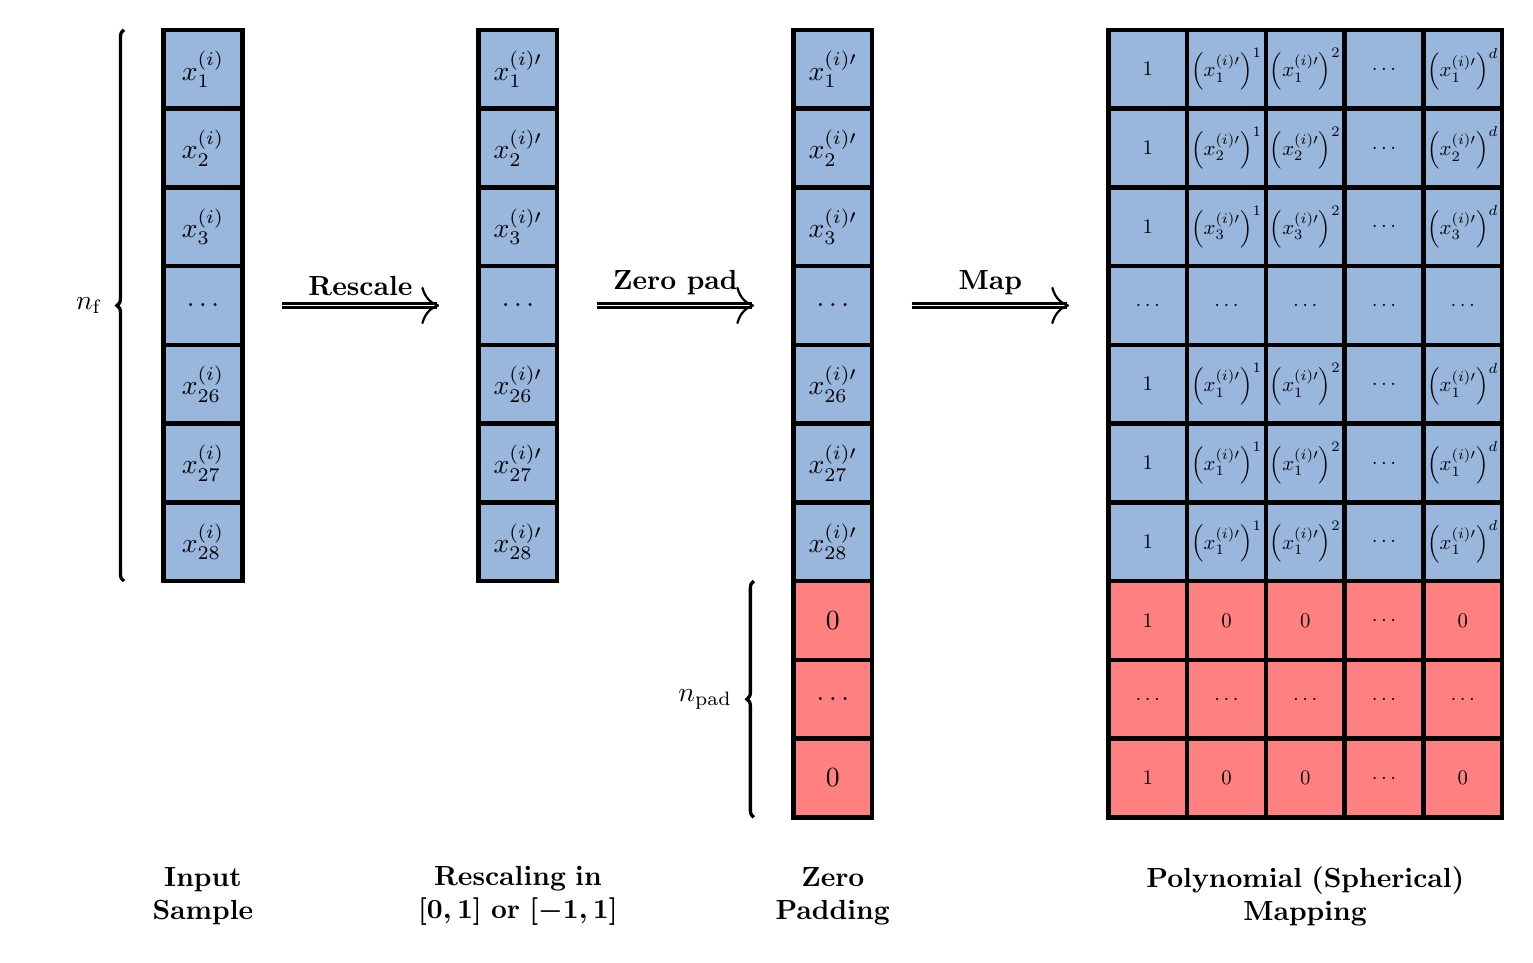
\begin{tikzpicture}[
        draw=black!50,
        node distance=0.3em,
        transform shape,scale=1.0
    ]
    
    \tikzstyle{annot} = [text width=12em, text centered]
    
    \def\XPA{0}
    \def\XPB{4}
    \def\XPC{8}
    \def\XPD{12}
    
    % upper
    \draw[ultra thick, draw=black, fill=white!60!cobalt] (\XPA,0) grid (\XPA+1,- 7) rectangle (\XPA,0);
    \draw[ultra thick, draw=black, fill=white!60!cobalt] (\XPB,0) grid (\XPB+1,- 7) rectangle (\XPB,0);
    \draw[ultra thick, draw=black, fill=white!60!cobalt] (\XPC,0) grid (\XPC+1,- 7) rectangle (\XPC,0);
    \draw[ultra thick, draw=black, fill=white!60!cobalt] (\XPD,0) grid (\XPD+5,- 7) rectangle (\XPD,0);
    
    % pad
    \draw[ultra thick, draw=black, fill=white!50!red] (\XPC,-7) grid (\XPC+1,-10) rectangle (\XPC,-7);
    \draw[ultra thick, draw=black, fill=white!50!red] (\XPD,-7) grid (\XPD+5,-10) rectangle (\XPD,-7);
    
    % PA nodes
    \node (PA-1)  at (\XPA+0.5,- 0.5) {\( x^{(i)}_{1}  \)};
    \node (PA-2)  at (\XPA+0.5,- 1.5) {\( x^{(i)}_{2}  \)};
    \node (PA-3)  at (\XPA+0.5,- 2.5) {\( x^{(i)}_{3}  \)};
    \node (PA-D)  at (\XPA+0.5,- 3.5) {\( \dots  \)};
    \node (PA-26) at (\XPA+0.5,- 4.5) {\( x^{(i)}_{26} \)};
    \node (PA-27) at (\XPA+0.5,- 5.5) {\( x^{(i)}_{27} \)};
    \node (PA-28) at (\XPA+0.5,- 6.5) {\( x^{(i)}_{28} \)};
    
    % PB nodes
    \node (PB-1)  at (\XPB+0.5,- 0.5) {\( x^{(i)\prime}_{1}  \)};
    \node (PB-2)  at (\XPB+0.5,- 1.5) {\( x^{(i)\prime}_{2}  \)};
    \node (PB-3)  at (\XPB+0.5,- 2.5) {\( x^{(i)\prime}_{3}  \)};
    \node (PB-D)  at (\XPB+0.5,- 3.5) {\( \dots              \)};
    \node (PB-26) at (\XPB+0.5,- 4.5) {\( x^{(i)\prime}_{26} \)};
    \node (PB-27) at (\XPB+0.5,- 5.5) {\( x^{(i)\prime}_{27} \)};
    \node (PB-28) at (\XPB+0.5,- 6.5) {\( x^{(i)\prime}_{28} \)};
    
    % PC nodes
    \node (PC-1)  at (\XPC+0.5,- 0.5) {\( x^{(i)\prime}_{1}  \)};
    \node (PC-2)  at (\XPC+0.5,- 1.5) {\( x^{(i)\prime}_{2}  \)};
    \node (PC-3)  at (\XPC+0.5,- 2.5) {\( x^{(i)\prime}_{3}  \)};
    \node (PC-D)  at (\XPC+0.5,- 3.5) {\( \dots              \)};
    \node (PC-26) at (\XPC+0.5,- 4.5) {\( x^{(i)\prime}_{26} \)};
    \node (PC-27) at (\XPC+0.5,- 5.5) {\( x^{(i)\prime}_{27} \)};
    \node (PC-28) at (\XPC+0.5,- 6.5) {\( x^{(i)\prime}_{28} \)};
    \node (PC-P1) at (\XPC+0.5,- 7.5) {\( 0                  \)};
    \node (PC-PD) at (\XPC+0.5,- 8.5) {\( \dots              \)};
    \node (PC-P3) at (\XPC+0.5,- 9.5) {\( 0                  \)};
    
    % PD nodes
    \node[scale=0.75] (PD0-1)  at (\XPD+0.5,- 0.5) {\( 1     \)};
    \node[scale=0.75] (PD0-2)  at (\XPD+0.5,- 1.5) {\( 1     \)};
    \node[scale=0.75] (PD0-3)  at (\XPD+0.5,- 2.5) {\( 1     \)};
    \node[scale=0.75] (PD0-D)  at (\XPD+0.5,- 3.5) {\( \dots \)};
    \node[scale=0.75] (PD0-26) at (\XPD+0.5,- 4.5) {\( 1     \)};
    \node[scale=0.75] (PD0-27) at (\XPD+0.5,- 5.5) {\( 1     \)};
    \node[scale=0.75] (PD0-28) at (\XPD+0.5,- 6.5) {\( 1     \)};
    \node[scale=0.75] (PD0-P1) at (\XPD+0.5,- 7.5) {\( 1     \)};
    \node[scale=0.75] (PD0-PD) at (\XPD+0.5,- 8.5) {\( \dots \)};
    \node[scale=0.75] (PD0-P3) at (\XPD+0.5,- 9.5) {\( 1     \)};
    %%% PD1 nodes
    \node[scale=0.75] (PD1-1)  at (\XPD+1.5,- 0.5) {\( \qty(x^{(i)\prime}_{1})^{1}  \)};
    \node[scale=0.75] (PD1-2)  at (\XPD+1.5,- 1.5) {\( \qty(x^{(i)\prime}_{2})^{1}  \)};
    \node[scale=0.75] (PD1-3)  at (\XPD+1.5,- 2.5) {\( \qty(x^{(i)\prime}_{3})^{1}  \)};
    \node[scale=0.75] (PD1-D)  at (\XPD+1.5,- 3.5) {\( \dots                        \)};
    \node[scale=0.75] (PD1-26) at (\XPD+1.5,- 4.5) {\( \qty(x^{(i)\prime}_{1})^{1}  \)};
    \node[scale=0.75] (PD1-27) at (\XPD+1.5,- 5.5) {\( \qty(x^{(i)\prime}_{1})^{1}  \)};
    \node[scale=0.75] (PD1-28) at (\XPD+1.5,- 6.5) {\( \qty(x^{(i)\prime}_{1})^{1}  \)};
    \node[scale=0.75] (PD1-P1) at (\XPD+1.5,- 7.5) {\( 0                            \)};
    \node[scale=0.75] (PD1-PD) at (\XPD+1.5,- 8.5) {\( \dots                        \)};
    \node[scale=0.75] (PD1-P3) at (\XPD+1.5,- 9.5) {\( 0                            \)};
    %%% PD2 nodes
    \node[scale=0.75] (PD2-1)  at (\XPD+2.5,- 0.5) {\( \qty(x^{(i)\prime}_{1})^{2}  \)};
    \node[scale=0.75] (PD2-2)  at (\XPD+2.5,- 1.5) {\( \qty(x^{(i)\prime}_{2})^{2}  \)};
    \node[scale=0.75] (PD2-3)  at (\XPD+2.5,- 2.5) {\( \qty(x^{(i)\prime}_{3})^{2}  \)};
    \node[scale=0.75] (PD2-D)  at (\XPD+2.5,- 3.5) {\( \dots                        \)};
    \node[scale=0.75] (PD2-26) at (\XPD+2.5,- 4.5) {\( \qty(x^{(i)\prime}_{1})^{2}  \)};
    \node[scale=0.75] (PD2-27) at (\XPD+2.5,- 5.5) {\( \qty(x^{(i)\prime}_{1})^{2}  \)};
    \node[scale=0.75] (PD2-28) at (\XPD+2.5,- 6.5) {\( \qty(x^{(i)\prime}_{1})^{2}  \)};
    \node[scale=0.75] (PD2-P1) at (\XPD+2.5,- 7.5) {\( 0                            \)};
    \node[scale=0.75] (PD2-PD) at (\XPD+2.5,- 8.5) {\( \dots                        \)};
    \node[scale=0.75] (PD2-P3) at (\XPD+2.5,- 9.5) {\( 0                            \)};
    %%% PD dots nodes
    \node[scale=0.75] (PD-D) at (\XPD+3.5,- 0.5) {\( \dots \)};
    \node[scale=0.75] (PD-D) at (\XPD+3.5,- 1.5) {\( \dots \)};
    \node[scale=0.75] (PD-D) at (\XPD+3.5,- 2.5) {\( \dots \)};
    \node[scale=0.75] (PD-D) at (\XPD+3.5,- 3.5) {\( \dots \)};
    \node[scale=0.75] (PD-D) at (\XPD+3.5,- 4.5) {\( \dots \)};
    \node[scale=0.75] (PD-D) at (\XPD+3.5,- 5.5) {\( \dots \)};
    \node[scale=0.75] (PD-D) at (\XPD+3.5,- 6.5) {\( \dots \)};
    \node[scale=0.75] (PD-D) at (\XPD+3.5,- 7.5) {\( \dots \)};
    \node[scale=0.75] (PD-D) at (\XPD+3.5,- 8.5) {\( \dots \)};
    \node[scale=0.75] (PD-D) at (\XPD+3.5,- 9.5) {\( \dots \)};
    %%% PDD nodes
    \node[scale=0.75] (PDD-1)  at (\XPD+4.5,- 0.5) {\( \qty(x^{(i)\prime}_{1})^{d}  \)};
    \node[scale=0.75] (PDD-2)  at (\XPD+4.5,- 1.5) {\( \qty(x^{(i)\prime}_{2})^{d}  \)};
    \node[scale=0.75] (PDD-3)  at (\XPD+4.5,- 2.5) {\( \qty(x^{(i)\prime}_{3})^{d}  \)};
    \node[scale=0.75] (PDD-D)  at (\XPD+4.5,- 3.5) {\( \dots                        \)};
    \node[scale=0.75] (PDD-26) at (\XPD+4.5,- 4.5) {\( \qty(x^{(i)\prime}_{1})^{d}  \)};
    \node[scale=0.75] (PDD-27) at (\XPD+4.5,- 5.5) {\( \qty(x^{(i)\prime}_{1})^{d}  \)};
    \node[scale=0.75] (PDD-28) at (\XPD+4.5,- 6.5) {\( \qty(x^{(i)\prime}_{1})^{d}  \)};
    \node[scale=0.75] (PDD-P1) at (\XPD+4.5,- 7.5) {\( 0                            \)};
    \node[scale=0.75] (PDD-PD) at (\XPD+4.5,- 8.5) {\( \dots                        \)};
    \node[scale=0.75] (PDD-P3) at (\XPD+4.5,- 9.5) {\( 0                            \)};
    
    % PA->PB
    \draw[double,->, thick, black] (\XPA+1.5, -3.5) -- (\XPB-0.5, -3.5) node[midway, anchor=south, align=center] {\textbf{Rescale}};
    
    % PB->PC
    \draw[double,->, thick, black] (\XPB+1.5, -3.5) -- (\XPC-0.5, -3.5) node[midway, anchor=south, align=center] {\textbf{Zero pad}};
    
    % PC->PD
    \draw[double,->, thick, black] (\XPC+1.5, -3.5) -- (\XPD-0.5, -3.5) node[midway, anchor=south, align=center] {\textbf{Map}};
    
    
    % underbraces
    \draw[
        very thick,
        decoration={
            brace,
            mirror,
            raise=0.1
        },
        decorate,
        black
    ] (-0.5,0) -- (-0.5,-7) node [midway, anchor=west, xshift=-0.75cm] {\( n_{\mathrm{f}} \)};
    
    \draw[
        very thick,
        decoration={
            brace,
            mirror,
            raise=0.1
        },
        decorate,
        black
    ] (-0.5+8,-7) -- (-0.5+8,-10) node [midway, anchor=west, xshift=-1.1cm] {\( n_{\mathrm{pad}} \)};
    
    
    % annotations
    \node[annot, below of=PA-28, node distance=4.5cm]  (PA-TEXT) {\textbf{Input\\Sample}};
    \node[annot, below of=PB-28, node distance=4.5cm]  (PB-TEXT) {\textbf{Rescaling in\\\( \boldsymbol{[0,1]} \) or \( \boldsymbol{[-1,1]} \)}};
    \node[annot, below of=PC-28, node distance=4.5cm]  (PC-TEXT) {\textbf{Zero\\Padding}};
    \node[annot, below of=PD2-28, node distance=4.5cm] (PC-TEXT) {\textbf{Polynomial (Spherical)\\Mapping}};
\end{tikzpicture}



\end{document}